%%%%%%%%%%%%%%%%%%%%%%%%%%%%%%%%%%%%%%%%%%%%%%%%%%%%%%%%%%%%%%%%%%%%%%%%%%%%%%%%
%2345678901234567890123456789012345678901234567890123456789012345678901234567890
%        1         2         3         4         5         6         7         8

\documentclass[letterpaper, 10 pt, conference]{ieeeconf}  % Comment this line out
                                                          % if you need a4paper
%\documentclass[a4paper, 10pt, conference]{ieeeconf}      % Use this line for a4
                                                          % paper

\IEEEoverridecommandlockouts                              % This command is only
                                                          % needed if you want to
                                                          % use the \thanks command
\overrideIEEEmargins
% See the \addtolength command later in the file to balance the column lengths
% on the last page of the document

\usepackage[utf8]{inputenc}
\usepackage[T1]{fontenc}
\usepackage{listings}
\usepackage{xcolor}
\usepackage{listings}
\usepackage{graphicx}
\usepackage{xparse}
\usepackage{threeparttable}
\usepackage{array}
\usepackage{tabularx}
\usepackage{subcaption}
\usepackage{tablefootnote}
\newcolumntype{Y}{>{\centering\arraybackslash}X}
\newcolumntype{L}{>{\raggedleft\arraybackslash}p{.2in}}
\newcolumntype{R}{>{\raggedright\arraybackslash}p{.2in}}
\NewDocumentCommand{\codeword}{v}{%
\texttt{\textcolor{black}{#1}}%
}

\lstset{language=C,keywordstyle={\bfseries \color{blue}}}

% The following packages can be found on http:\\www.ctan.org
%\usepackage{graphics} % for pdf, bitmapped graphics files
%\usepackage{epsfig} % for postscript graphics files
%\usepackage{mathptmx} % assumes new font selection scheme installed
%\usepackage{mathptmx} % assumes new font selection scheme installed
%\usepackage{amsmath} % assumes amsmath package installed
%\usepackage{amssymb}  % assumes amsmath package installed
\usepackage{hyperref}
\usepackage{multicol}
\title{\LARGE
\textbf{Price Prediction with Neural Networks:\\ Time Series Forecast meets Deep Learning}\\
\Large
\textit{Prospectus}\\
\Large
CSC 240 Final Project
}

%\author{ \parbox{3 in}{\centering Huibert Kwakernaak*
%         \thanks{*Use the $\backslash$thanks command to put information here}\\
%         Faculty of Electrical Engineering, Mathematics and Computer Science\\
%         University of Twente\\
%         7500 AE Enschede, The Netherlands\\
%         {\tt\small h.kwakernaak@autsubmit.com}}
%         \hspace*{ 0.5 in}
%         \parbox{3 in}{ \centering Pradeep Misra**
%         \thanks{**The footnote marks may be inserted manually}\\
%        Department of Electrical Engineering \\
%         Wright State University\\
%         Dayton, OH 45435, USA\\
%         {\tt\small pmisra@cs.wright.edu}}
%}
\author{Minh Khoi Nguyen Do, Vuong Ho, Chuqin Wu, Quianwen Fu}


\begin{document}



\maketitle
\thispagestyle{empty}
\pagestyle{empty}


%%%%%%%%%%%%%%%%%%%%%%%%%%%%%%%%%%%%%%%%%%%%%%%%%%%%%%%%%%%%%%%%%%%%%%%%%%%%%%%%
\begin{abstract}
For the final project of CSC240, we look to apply deep learning techniques in the subject of time series analysis and analyze its performance in this type of task, and possibly compare their accuracy against autoregressive methods, which are algorithms specially developed for time series data. Specifically, we look at whether neural networks can be applied in the financial sectors by using a variety of networks such as bidirectional RNN, GRU, and LSTM to predict future prices of Microsoft stocks, Bitcoin, and similar datasets. We have also prepared and generated artificial time series datasets that simulates reality to see how deep learning can be applied in this kind of task. Here in this prospectus, we discuss our plans to approach this final project.

\end{abstract}


%%%%%%%%%%%%%%%%%%%%%%%%%%%%%%%%%%%%%%%%%%%%%%%%%%%%%%%%%%%%%%%%%%%%%%%%%%%%%%%%
\section{INTRODUCTION}
\subsection{About time series}
    From every day's temperature to stock market price, time series data appears everywhere in every parts of our life. As such, it is inevitable that each one of us has wondered at least once about what tomorrow's temperature will be, or whether this cryptocurrency that we have invested will make us appear in the next Forbes 30 under 30, or will it just pull us deeper in the red. The subject of time series forecasting has been widely researched back in the later half of 20th century, with many algorithms having been developed, and widely used, for this kind of task, most notably autoregressive methods.

\subsection{Deep learning in time series forecasting}
    With autoregerssive methods seem to be the go-to algorithms for this task, our team decides to take a step back and approach this problem in a different way: using deep learning. For our final project, we are interested in seeing whether deep learning algorithms can be used for the price prediction task in financial datasets, the extent of which some techniques can be used and their effectiveness, and how well they work in both real-life time series dataset and artificial ones.

\section{OUR APPROACH}
In this section, we will elaborate how we will tackle the goal we have set out in the Introduction section, what deep learning techniques we will be using, and how we will conduct our analysis.

\subsection{Deep learning models}
    In time series dataset, any piece of data at any given point in time may depend on the data before and after it, which means that context matters a lot in determining a value in time. Due to this property of time series data, recurrent neural networks seem to be best fit for this job, and so we will be applying this type of networks along with their variations for our analysis. Specifically, we will be using in total four recurrent-type neural networks which are: 
    \begin{itemize}
        \item Traditional RNN
        \item Bidirectional RNN
        \item GRU, or RNN with forget gates
        \item LSTM
    \end{itemize}
    which we will apply on a variety of financial datasets and compare their performance in each of the datasets.

\subsection{Datasets and some analysis}
    To test the performance of the four deep learning models we have listed above, we decide to use four financial datasets that come from three different fields, and also two more artificial datasets we generate with certain constraints. We prepare four real-life datasets which come from slightly different financial contexts, whose subfields and metadata we listed in the table below:

    \begin{table}[h!] \centering
        \caption{Datasets }
        \begin{threeparttable}
                \begin{tabular}{|c||c|c|}
                    \hline
                    Dataset name & Field & Source\\
                    \hline
                    Microsoft Stock Prices & Stock market & Kaggle\tablefootnote{\url{https://www.kaggle.com/vijayvvenkitesh/microsoft-stock-time-series-analysis}}\\
                    S\&P 500 Index & Stock market & DataHub\tablefootnote{\url{https://datahub.io/core/s-and-p-500}}\\
                    Europe Crude Oil Prices & Natural resources & FRED Economic Data\tablefootnote{\url{https://fred.stlouisfed.org/series/DCOILBRENTEU}}\\
                    Bitcoin Prices & Cryptocurrency & Kaggle\tablefootnote{\url{https://www.kaggle.com/sudalairajkumar/cryptocurrencypricehistory}}\\
                    \hline
                \end{tabular}
        \end{threeparttable}
    \end{table}

    With the four datasets belonging into slightly different subfields of the financial world, we can reliably compare our prediction accuracy of each models we use and apply our findings to generalize without biases. This following subsections detail some analysis on the above four datasets:

    \subsubsection{Microsoft Stock prices} For this dataset, we decide to go with the close stock prices of Microsoft (MSFT on NASDAQ) from 2015-04-01 to 2021-03-3. Here we graph the values of Microsoft Stock prices over time in Fig. 1:
    \begin{figure}[thpb]
        \centering
        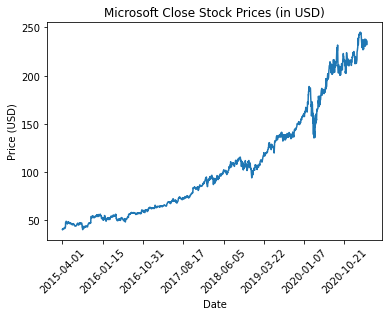
\includegraphics[width=8cm]{1.png}
        \caption{Microsoft (MSFT) close stock prices (in USD) over time.}
        \label{figurelabel}
     \end{figure}
    
    \subsubsection{S\&P 500 Index} The Standard \& Poor 500 Index (S\&P 500) is a stock market index tracking the performance of 500 large companies listed on stock exchanges in the United States\footnote{Wikipedia}, and the dataset that we have contains index from 1871-01-01 to 2018-04-01. Here we graph the values of the S\&P 500 Index over time in Fig. 2:

    \begin{figure}[thpb]
        \centering
        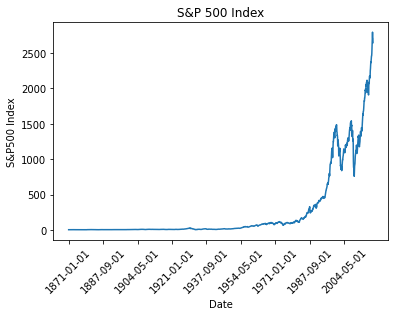
\includegraphics[width=8cm]{2.png}
        \caption{S\&P 500 Index over time.}
        \label{figurelabel}
     \end{figure}

     \subsubsection{Europe Crude Oil Prices} The dataset contains the crude oil prices (in USD) of Europe from 2015-11-02 to 2021-11-01. Here we graph the values of the Europe crude oil prices over time in Fig. 3:

     \begin{figure}[thpb]
         \centering
         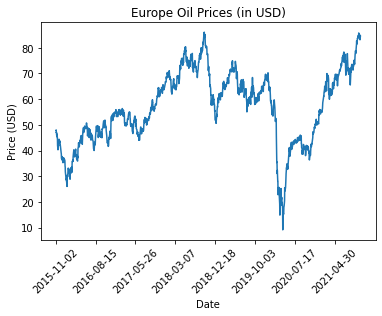
\includegraphics[width=8cm]{3.png}
         \caption{Europe crude oil prices (in USD) over time.}
         \label{figurelabel}
      \end{figure}

      \subsubsection{Bitcoin Prices} The main dataset from Kaggle offer prices of many different cryptocurrency; however, we decided to go with Bitcoin since it seems to be the most popular one currently as of 2021. The dataset contains Bitcoin prices (in USD) at close from 2013-04-29 to 2021-07-06. Here we graph the values of the Bitcoin prices at close over time in Fig. 4:

      \begin{figure}[thpb]
          \centering
          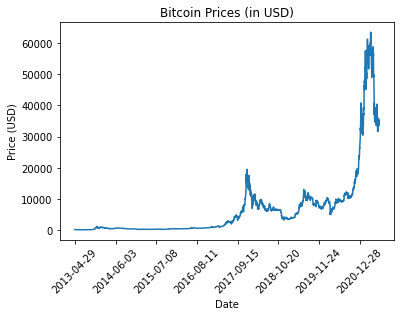
\includegraphics[width=8cm]{4.png}
          \caption{Bitcoin prices (in USD) at close over time.}
          \label{figurelabel}
       \end{figure}

    Besides the real-life datasets listed above, we have also created an algorithm that generated artificial time series dataset, and would apply our neural networks on two which will be created during the course of our final project. Fig 5 and 6 showcase two artificial datasets that were generated by our methods.
    \begin{figure}[thpb]
        \centering
        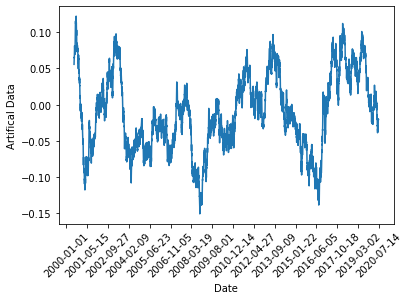
\includegraphics[width=8cm]{5.png}
        \caption{Generated time series dataset example 1.}
        \label{figurelabel}
     \end{figure}
     \begin{figure}[thpb]
        \centering
        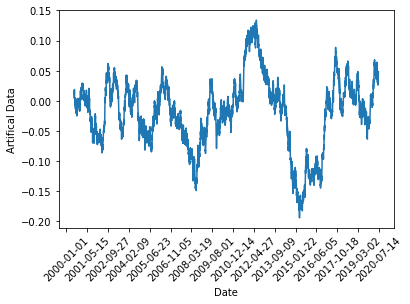
\includegraphics[width=8cm]{6.png}
        \caption{Generated time series dataset example 2.}
        \label{figurelabel}
     \end{figure}
\section{EXPECTATIONS \& TIMELINE}

    \subsection{Expectations}
    The goal we have set out for this final project is to examine whether deep learning techniques can be used in place of autoregressive methods in this price prediction challenge. By using the four neural networks on the datasets that we have introduced above, we hope to be able to gain insights on the effectiveness of deep learning in time series analysis and forecasting, and explore which neural networks can best be used for certain types of datasets by conducting a series of statistical analysis at the results of the prediction. With everything we have set up above, we believe that we will be able to produce a meaningful report out of this final project.

    \subsection{Timeline}
    We have created a detailed schedule of our final project, with the following milestones:
    \begin{itemize}
        \item Nov 6-9: Complete the analysis of the 4 real-life datasets, as well as the algorithms to generate artificial data.
        \item Nov 10-12: Gather dataset analysis and write prospectus.
        \item Nov 13-19: Implement the 4 neural networks above.
        \item Nov 20-25: Train the 4 neural networks on the datasets and conduct analysis on the results.
        \item Nov 26-29: Compile the analysis results, do further analysis between the different neural network, and create presentation material.
        \item Nov 30-Dec 4: Conduct further analysis in the results and write the Final Essay.
        \item Dec 4-7: Final compilation and revision of the Final Essay before submission. 
    \end{itemize}

    We also hold a weekly meeting up until the last day of the final project in order to report on our progress and also to discuss on current approach. For the division of labor, we have set up as follows:

    \subsubsection{Dataset Analysis} For this section, Vuong and Minh Khoi will work on analyzing the Bitcoin and the Europe Crude Oil price datasets, while Chuqin and Quianwen work on Microsoft Stock prices and S\&P 500 Index.

    \subsubsection{Prospectus} Vuong will be responsible for writing the prospectus, which is what you are reading right now.

    \subsubsection{Neural network implementation} We have split up the four neural networks implementation responsiblity as detailed in the following table:
    \begin{table}[h!] \centering
        \caption{Datasets }
        \begin{threeparttable}
                \begin{tabular}{|c|c|}
                    \hline
                    Neural Network Name & Implementer\\
                    \hline
                    Traditional RNN & Quianwen\\
                    Bidirectional RNN & Vuong\\
                    GRU & Chuqin\\
                    LSTM & Minh Khoi\\
                    \hline
                \end{tabular}
        \end{threeparttable}
    \end{table}

    Each person will also be responsible for applying their implementation to the datasets, as well as conducting analysis on the results. With their results, each person will go ahead and write up their own report and analysis, which will be pieced together in the presentation and the final essay.

    \subsubsection{Presentation \& Final Essay} As mentioned above, each person will be responsible for their chosen neural networks, both writing up the materials and presentation slots. The general analysis for all four neural networks will be done by all four members. The final essay will be written up and compiled from the four analysis by Vuong.

\section{CONCLUSION}
    In this prospectus, we have laid out how we are going to approach the final project with the idea of exploring the possibilities of deep learning in time series forecasting, specifically price prediction. By taking a look at four recurrent neural network structures and using them for prediction in both real-life and artificial financial datasets, we hope to be able to analyze the performance of deep learning in price prediction, and this, we believe, will open paths to more research on such methods in time series forecasting with deep learning. 

\end{document}
